\subsubsection{Randomnesss} \label{sec:lag_res_random}
In order to quantitatively detect the patchiness present in the spatial distribution of the cells, a meaningful quantity which can be defined is the \textit{deviation between mean and variance}, which is an estimator of the deviation from randomness. The Poisson distribution is \autocite[chapter 8.5]{loreti2006teoria}
\[ P(x;\lambda) = \frac{e^\lambda \lambda^{-x}}{x!} \]
and its mean $\mu$ and variance $\sigma^2$ are
\[ \mu = \sigma^2 = \lambda \]
This distribution models rare, random events occurrence. Evaluating the relative difference between these two values relative to the mean gives an estimate of the deviation from the Poisson distribution, and thus from randomness. \\
For an analysis of the simulated structure, the particles have been grouped in ``boxes'' of varying size, then the number of particles in each box has been sampled, and put in a histogram which looks at the distribution of the number of particles per box along the vertical direction.
The results can be seen in \autoref{fig:lag_res_random}: the binning on vertical direction is kept constant, in order to notice the horizontal clustering structure. While increasing the dimension of horizontal bins, the deviation from randomness accentuate, to reach a maximum at $\sim\frac{1}{3}$ of the simulation box size, and then decrease. When the binning is very dense, the boxes probe a length which is too small to detect structure; on the contrary, when the binning reaches a size similar to the simulation box, the irregularities are averaged out. This means that the characteristic size of the patches is comparable to the binning size of the higher curve, that is, approximately a third of the side length. 

\begin{figure}[h]
    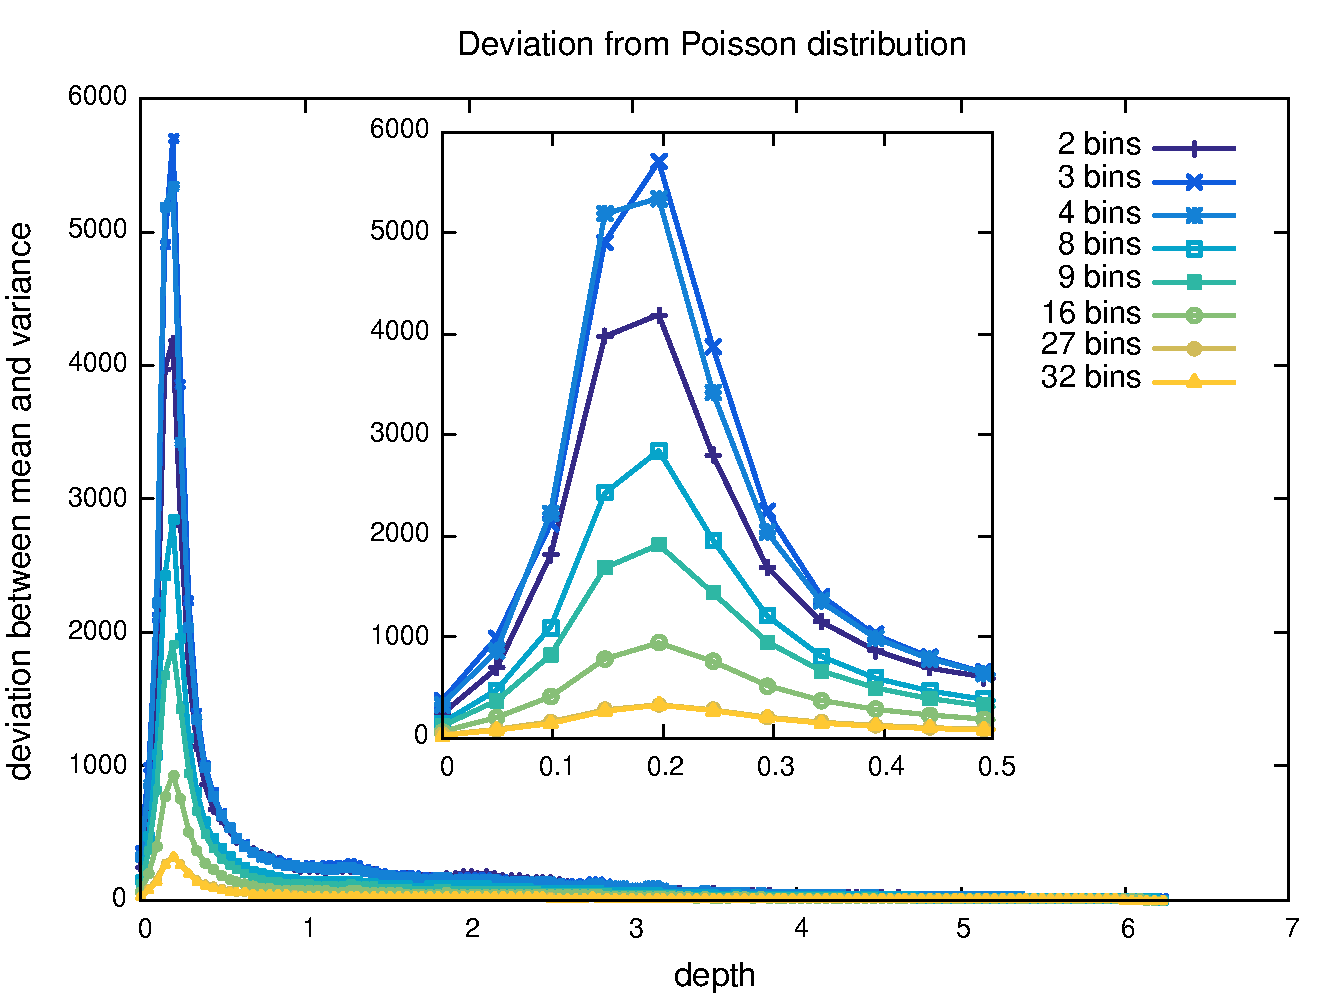
\includegraphics[width=\textwidth]{data/3D_model/run2/dev_poisson_1}
    \caption{The relative difference between mean and variance for the particles distribution at different binnings in the horizontal directions. The deviation from Poisson's distribution increases while increasing the bin size, having a maximum at $\sim\frac{1}{3}$ of the simulation box and then decreasing.}
    \label{fig:lag_res_random}
\end{figure}